% Options for packages loaded elsewhere
\PassOptionsToPackage{unicode}{hyperref}
\PassOptionsToPackage{hyphens}{url}
\PassOptionsToPackage{dvipsnames,svgnames,x11names}{xcolor}
%
\documentclass[
]{article}
\usepackage{amsmath,amssymb}
\usepackage{iftex}
\ifPDFTeX
  \usepackage[T1]{fontenc}
  \usepackage[utf8]{inputenc}
  \usepackage{textcomp} % provide euro and other symbols
\else % if luatex or xetex
  \usepackage{unicode-math} % this also loads fontspec
  \defaultfontfeatures{Scale=MatchLowercase}
  \defaultfontfeatures[\rmfamily]{Ligatures=TeX,Scale=1}
\fi
\usepackage{lmodern}
\ifPDFTeX\else
  % xetex/luatex font selection
\fi
% Use upquote if available, for straight quotes in verbatim environments
\IfFileExists{upquote.sty}{\usepackage{upquote}}{}
\IfFileExists{microtype.sty}{% use microtype if available
  \usepackage[]{microtype}
  \UseMicrotypeSet[protrusion]{basicmath} % disable protrusion for tt fonts
}{}
\makeatletter
\@ifundefined{KOMAClassName}{% if non-KOMA class
  \IfFileExists{parskip.sty}{%
    \usepackage{parskip}
  }{% else
    \setlength{\parindent}{0pt}
    \setlength{\parskip}{6pt plus 2pt minus 1pt}}
}{% if KOMA class
  \KOMAoptions{parskip=half}}
\makeatother
\usepackage{xcolor}
\usepackage[left=2cm,right=2cm,top=1cm,bottom=1.5cm]{geometry}
\usepackage{longtable,booktabs,array}
\usepackage{calc} % for calculating minipage widths
% Correct order of tables after \paragraph or \subparagraph
\usepackage{etoolbox}
\makeatletter
\patchcmd\longtable{\par}{\if@noskipsec\mbox{}\fi\par}{}{}
\makeatother
% Allow footnotes in longtable head/foot
\IfFileExists{footnotehyper.sty}{\usepackage{footnotehyper}}{\usepackage{footnote}}
\makesavenoteenv{longtable}
\usepackage{graphicx}
\makeatletter
\def\maxwidth{\ifdim\Gin@nat@width>\linewidth\linewidth\else\Gin@nat@width\fi}
\def\maxheight{\ifdim\Gin@nat@height>\textheight\textheight\else\Gin@nat@height\fi}
\makeatother
% Scale images if necessary, so that they will not overflow the page
% margins by default, and it is still possible to overwrite the defaults
% using explicit options in \includegraphics[width, height, ...]{}
\setkeys{Gin}{width=\maxwidth,height=\maxheight,keepaspectratio}
% Set default figure placement to htbp
\makeatletter
\def\fps@figure{htbp}
\makeatother
\setlength{\emergencystretch}{3em} % prevent overfull lines
\providecommand{\tightlist}{%
  \setlength{\itemsep}{0pt}\setlength{\parskip}{0pt}}
\setcounter{secnumdepth}{-\maxdimen} % remove section numbering
\usepackage{wrapfig}
\usepackage{graphicx}
\usepackage{titlesec}
\titlespacing*{\section}{0pt}{\baselineskip}{0.1\baselineskip}
\titlespacing*{\subsection}{0pt}{\baselineskip}{0.1\baselineskip}
\titlespacing*{\subsubsection}{0pt}{\baselineskip}{0.1\baselineskip}
\usepackage{fancyhdr}
\pagestyle{fancy}
\fancyhf{}
\fancyfoot[R]{This CV is prepared using R Markdown}
\renewcommand{\headrulewidth}{0pt}
\usepackage{etoolbox}
\AtBeginEnvironment{table}{\vspace{-0.1\baselineskip}}
\ifLuaTeX
  \usepackage{selnolig}  % disable illegal ligatures
\fi
\usepackage{bookmark}
\IfFileExists{xurl.sty}{\usepackage{xurl}}{} % add URL line breaks if available
\urlstyle{same}
\hypersetup{
  colorlinks=true,
  linkcolor={Maroon},
  filecolor={Maroon},
  citecolor={Blue},
  urlcolor={blue},
  pdfcreator={LaTeX via pandoc}}

\author{}
\date{\vspace{-2.5em}}

\begin{document}

\pagenumbering{gobble}
\begin{centering}

\Large

{\bf PRAKASH LAMICHHANE}

\normalsize
Research Officer/Data Ananlyst/Ecologist

\end{centering}

\normalsize

Email:
\href{mailto:forester.prakash@gmail.com}{\nolinkurl{forester.prakash@gmail.com}}
\textbar{} Phone: +977-9845228896 \textbar{} GitHub:
\href{https://github.com/foresterprakash}{foresterprakash} \textbar{}
LinkedIn:
\href{https://www.linkedin.com/in/PrakashLamichhane}{PrakashLamichhane}
\textbar{} ORCID:
\href{https://orcid.org/0000-0002-0355-0222}{0000-0002-0355-0222}

\section{\texorpdfstring{\underline{About Myself}}{}}\label{section}

\begin{wrapfigure}{r}{0.2\textwidth}
    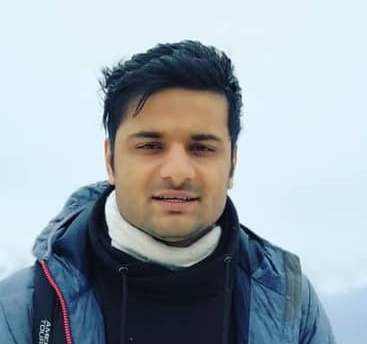
\includegraphics[width=0.2\textwidth]{Photo_Prakash.jpg}
\end{wrapfigure}

I am Prakash Lamichhane, a Research Officer, Data Analyst, and Ecologist
with a strong educational background in Forestry and Landscape Ecology.
My career spans practical experience in forest management and carbon
monitoring, driven by a passion for climate science and environmental
conservation efforts. I had a significant growth on data analysis and
statistical application in any sector data with mastering in MS Excel
and R programming in recent years. I am particularly interested in
advancing my academic growth in data science and statistical analysis
using R programming. I am looking forward to learn from an academic
environment to develop data driven approaches to understand the impact
of natural disaster on people and ecosystem. Specifically, my research
interest encompasses developing an ecosystem service framework linking
cultural heritage and promoting disaster resilient communities.

\section{\texorpdfstring{\underline{Education}}{}}\label{section-1}

\begin{longtable}[]{@{}
  >{\raggedright\arraybackslash}p{(\columnwidth - 6\tabcolsep) * \real{0.1392}}
  >{\raggedright\arraybackslash}p{(\columnwidth - 6\tabcolsep) * \real{0.4937}}
  >{\raggedright\arraybackslash}p{(\columnwidth - 6\tabcolsep) * \real{0.2278}}
  >{\raggedright\arraybackslash}p{(\columnwidth - 6\tabcolsep) * \real{0.1392}}@{}}
\toprule\noalign{}
\begin{minipage}[b]{\linewidth}\raggedright
Duration
\end{minipage} & \begin{minipage}[b]{\linewidth}\raggedright
Course
\end{minipage} & \begin{minipage}[b]{\linewidth}\raggedright
University
\end{minipage} & \begin{minipage}[b]{\linewidth}\raggedright
Country
\end{minipage} \\
\midrule\noalign{}
\endhead
\bottomrule\noalign{}
\endlastfoot
2017 - 2019 & M.Sc. Landscape Ecology and Nature Conservation &
University of Greifswald & Germany \\
& & & \\
2010 - 2013 & B.Sc. Forestry & Tribhuvan University & Nepal \\
& & & \\
2007 - 2009 & Technical Level in Forestry (I.Sc.) & Tribhuvan University
& Nepal \\
& & & \\
\end{longtable}

\section{\texorpdfstring{\underline{Work Experiences}}{}}\label{section-2}

\begin{longtable}[]{@{}
  >{\raggedright\arraybackslash}p{(\columnwidth - 2\tabcolsep) * \real{0.1867}}
  >{\raggedright\arraybackslash}p{(\columnwidth - 2\tabcolsep) * \real{0.8133}}@{}}
\toprule\noalign{}
\begin{minipage}[b]{\linewidth}\raggedright
Year
\end{minipage} & \begin{minipage}[b]{\linewidth}\raggedright
Affiliation
\end{minipage} \\
\midrule\noalign{}
\endhead
\bottomrule\noalign{}
\endlastfoot
2017 - 2019 & M.Sc. Landscape Ecology and Nature Conservation,
Greifswald University \\
& \\
2019 - 2023 & Assistant Research Officer, Forest Survey and Carbon
Monitoring Section under FRTC \\
& \\
2023 - Present & Research Officer, Climate Change Management Division,
MOFE \\
& \\
Part-time & Lecturer, Natural Resource Economics, Kathmandu Forestry
College \\
& \\
\end{longtable}

\section{\texorpdfstring{\underline{Major Skills}}{}}\label{section-3}

\begin{itemize}
\tightlist
\item
  National Forest data analysis and Reporting
\item
  Mastering MS. Excel and R programming
\item
  Carbon accounting and MRV process
\item
  Uncertainty Estimation and Sensitivity Analysis
\item
  Data Science with Python
\item
  GIS Tools (QGIS, ARCGIS, Google Earth Engine etc.)
\item
  Integrated Development Environments (IDEs)(i.e., R Studio, VS code,
  Pycharm, Jupyter Notebook, Collect Earth Online etc.).
\end{itemize}

\newpage

\section{\texorpdfstring{\underline{Major Job-Related Trainings as Trainee}}{}}\label{section-4}

\begin{longtable}[]{@{}
  >{\raggedright\arraybackslash}p{(\columnwidth - 6\tabcolsep) * \real{0.1765}}
  >{\raggedright\arraybackslash}p{(\columnwidth - 6\tabcolsep) * \real{0.3529}}
  >{\raggedright\arraybackslash}p{(\columnwidth - 6\tabcolsep) * \real{0.3235}}
  >{\raggedright\arraybackslash}p{(\columnwidth - 6\tabcolsep) * \real{0.1471}}@{}}
\toprule\noalign{}
\begin{minipage}[b]{\linewidth}\raggedright
Duration
\end{minipage} & \begin{minipage}[b]{\linewidth}\raggedright
Entitled
\end{minipage} & \begin{minipage}[b]{\linewidth}\raggedright
Organizers
\end{minipage} & \begin{minipage}[b]{\linewidth}\raggedright
Reference
\end{minipage} \\
\midrule\noalign{}
\endhead
\bottomrule\noalign{}
\endlastfoot
23-27 May, 2022 & Training on Unbiased Area Estimation and Uncertainty
Estimation for Forest Activity Data & USAID,USFS,SilvaCarbon &
\href{https://crystal-wespestad.com/}{Crystal Westespad} \\
& & & \\
22- 26 August, 2022 & Development of National Landcover Monitoring
System for Nepal & International Center for Integrated Mountain
Development (ICIMOD) SERVIR-HKH initiative &
\href{https://www.icimod.org/team/kabir-uddin}{kabir Uddin} \\
& & & \\
10 October - 11 November, 2022 & On the Job training on Forest Carbon
Stock Measurement using Earth Observation Data & International Center
for Integrated Mountain Development (ICIMOD) SERVIR-HKH initiative &
\href{https://www.icimod.org/team/rajesh-bahadur-thapa/}{Rajesh Bahadur
Thapa} \\
& & & \\
12 May - 13 August 2023 & Data Science with Python &
\href{https://broadwayinfosys.com/}{Broadways Infosys Pvt.Ltd.} &
\href{https://www.linkedin.com/in/uttam-adhikari-30a53660/?originalSubdomain=np}{Uttam
Adhikari} \\
& & & \\
21- 25 January 2024 & FCPF and ART TREES: Technical Training Workshop on
REDD+ Emission Reduction Measurement, Reporting and Verification
(30hours) & \href{https://redd.gov.np/}{REDD + Implemmentation
center},\href{https://www.silvacarbon.org/}{SilvaCarbon},
\href{https://www.forestcarbonpartnership.org/sites/default/files/documents/nepal_ermr_ghg_accounting_nov_2023_final.pdf}{FCPF},
\href{https://www.worldbank.org/en/home}{The WorldBank Group Nepal} &
\href{https://www.linkedin.com/in/german-obando-vargas-24b70319/?originalSubdomain=cr}{German
Obando - Vargas} \\
& & & \\
22-26 July 2024 & Earth Observation (LiDAR and GEDI) for forest
carbonstocks monitoring in Nepal & ICIMOD, FRTC,SilvaCarbon &
\href{https://www.icimod.org/team/rajesh-bahadur-thapa/}{Rajesh Bahadur
Thapa} and \href{https://www.linkedin.com/in/timothy-devereux/}{Tim
Devereux} \\
& & & \\
19 Aug - 6 September 2024 & Climate Action and Support Transparency
Training(CASTT) Programme on GHGs in Seoul,Republic of Korea &
\textbf{UNFCCC}and Green House Gas Inventory and Research Center, South
Korea & \href{https://www.linkedin.com/in/eunhae-jeong-248a40124/}{Jeong
Eun-hae,President, GIR Korea} \\
\end{longtable}

\section{\texorpdfstring{\underline{Major Job-Related Trainings as Trainer}}{}}\label{section-5}

\begin{longtable}[]{@{}
  >{\raggedright\arraybackslash}p{(\columnwidth - 4\tabcolsep) * \real{0.2188}}
  >{\raggedright\arraybackslash}p{(\columnwidth - 4\tabcolsep) * \real{0.5000}}
  >{\raggedright\arraybackslash}p{(\columnwidth - 4\tabcolsep) * \real{0.2812}}@{}}
\toprule\noalign{}
\begin{minipage}[b]{\linewidth}\raggedright
Duration
\end{minipage} & \begin{minipage}[b]{\linewidth}\raggedright
Entitled
\end{minipage} & \begin{minipage}[b]{\linewidth}\raggedright
Organization
\end{minipage} \\
\midrule\noalign{}
\endhead
\bottomrule\noalign{}
\endlastfoot
Regular From 2022 & MS Excel and R Programming Trainer in &
\href{https://broadwayinfosys.com/}{Broadways Infosys} \\
14 - 21 Aug, 2023 & Training on Python Programming &
\href{https://frtc.gov.np/}{Forest Research and TRaining Center} \\
26 Sept - 5 Oct, 2023 & Statistical Data Analysis and Forest Mapping &
\href{https://frtc.gov.np/}{Forest Research and Training Center} \\
4-13 Feb, 2024 & Enhancing Capacity on R Programming for Data Analysis
and Carbon Accounting & \href{https://redd.gov.np/}{REDD+ Implementation
center} \\
\end{longtable}

\section{\texorpdfstring{\underline{Workshop and Seminar}}{}}\label{section-6}

\begin{enumerate}
\def\labelenumi{\arabic{enumi}.}
\tightlist
\item
  Cross Country knowledge Exchange on REDD plus program in Cambodia
  dated from 12/06/2022 to 19/06/2022 Phnom Penn, Siem Reip and Koh Kong
  province of Cambodia (ORAL PRESENTATION)
\item
  South-South Knowledge Exchange on Measurement, Monitoring, Reporting
  and Verification systems, FCPF CF ERPA Implementation dated from
  12/12/2022 -- 18/12/2022 -- Maputo, Mozambique.
\item
  Hands-on training workshop on transitioning to the ETF, including the
  preparation of the Biennial Transparency Report for Asia Region dated
  from 12/03/2024 to 15/03/2024 Singapore.
\item
  UN Climate Conference Bonn, Germany dated from 03/06/2024 to
  09/06/2024
\end{enumerate}

\newpage

\section{\texorpdfstring{\underline{Research Experience}}{}}\label{section-7}

\begin{enumerate}
\def\labelenumi{\arabic{enumi}.}
\tightlist
\item
  Preparation of National Landcover monitoring System (NLCMS) using
  RandomForestClassifier.
\item
  FRTC, 2020, A study of Opportunities and Constraints for Development
  of Private forestry Model in Mid-Hill Region of Nepal (A case study
  from Kavre and Kaski district of Nepal), Forest Research and Training
  Centre (FRTC), Babarmahal, Kathmandu, Nepal.
  \href{https://frtc.gov.np/uploads/files/Private\%20forest\%20Model(1).pdf}{Unpublished}
\item
  Preparation of Regional and National Forest Resource assessment
  (Involvement in field data collection, data analysis and report
  writing).
\item
  Involvement in generating activity data and emission factors for
  national emission reduction report for MRV purpose in coordination
  with FCPF and World Bank.
\end{enumerate}

\section{\texorpdfstring{\underline{Publications}}{}}\label{section-8}

\begin{enumerate}
\def\labelenumi{\arabic{enumi}.}
\tightlist
\item
  Aryal, S., Paudel, P., Bolakhe, S., Mahatara, D., \& Lamichhane, P.
  (2022). Evaluation of error and efficiency on tree height measurement
  using Abney's level, Rangefinder and Vertex IV. \emph{Indian Journal
  of Forestry}, 45(1), 1--8.
  \href{https://doi.org/10.54207/bsmps1000-2022-49P4F8}{DOI}
\item
  Parajuli, A., Gautam, A. P., Sharma, S., Lamichhane, P., Sharma, G.,
  Bist, B. S., Aryal, U., \& Basnet, R. (2022). A Strategy for involving
  community forest managers in effective forest fire management in
  Nepal. \emph{Banko Janakari}, 32(1), 41--51.
  \href{https://doi.org/10.3126/banko.v32i1.45476}{DOI}
\item
  Subedi, B., Lamichhane, P., Magar, L. K., \& Subedi, T. (2022).
  Aboveground carbon stocks and sequestration rates of forests under
  different management regimes in Churia region of Nepal. \emph{Banko
  Janakari}, 32(1), 15--24.
  \href{https://doi.org/10.3126/banko.v32i1.45442}{DOI}
\item
  Gautam, G. P., Aryal, R. R., \& Lamichhane, P. (2018). Restoration of
  degraded land through Moso bamboo (Phyllostachys pubescens) plantation
  in the Mid-hills of Nepal. \emph{Banko Janakari}, 150--153.
  \href{https://doi.org/10.3126/banko.v27i3.20560}{DOI}
\item
  Dhakal, R., et al.~(2023). Developing Stem Taper of Shorea Robusta in
  the Far-Western Terai of Nepal. \emph{Banko Janakari}, 33(2), 3--10.
  \href{https://doi.org/10.3126/banko.v33i2.58809}{DOI}
\end{enumerate}

\section{\texorpdfstring{\underline{References}}{}}\label{section-9}

\small

\begin{longtable}[]{@{}
  >{\raggedright\arraybackslash}p{(\columnwidth - 4\tabcolsep) * \real{0.3333}}
  >{\raggedright\arraybackslash}p{(\columnwidth - 4\tabcolsep) * \real{0.3333}}
  >{\raggedright\arraybackslash}p{(\columnwidth - 4\tabcolsep) * \real{0.3333}}@{}}
\toprule\noalign{}
\begin{minipage}[b]{\linewidth}\raggedright
Referee 1
\end{minipage} & \begin{minipage}[b]{\linewidth}\raggedright
Referee 2
\end{minipage} & \begin{minipage}[b]{\linewidth}\raggedright
Referee 3
\end{minipage} \\
\midrule\noalign{}
\endhead
\bottomrule\noalign{}
\endlastfoot
\textbf{Shiva Khanal PhD} & \textbf{Shes Kanta Bhandari PhD} &
\textbf{Buddi Sagar Poudel, PhD} \\
Western Sydney University,Australia & University of Western Australia &
Charles Sturt University,Australia \\
Under Secretary (Tech.), Climate Change Management Division (CCMD) &
Assistant Professor, Institute of Forestry, Tribhuvan University & Joint
Secretary, Climate Change Management Division (CCMD) \\
Ministry of Forests and Environment, Kathmandu, Nepal & \textbf{Research
Interests:} Forest Biometrics, Forest Growth and Yield Modelling,
Individual-based Modelling, Forest Inventory & Ministry of Forests and
Environment, Kathmandu, Nepal \\
\textbf{Google Scholar:}
\href{https://scholar.google.com/citations?user=XXXXXXXXXXXX}{Shiva
Khanal} & \textbf{Google Scholar:}
\href{https://scholar.google.com/citations?user=k9sUEZkAAAAJ}{Shes Kanta
Bhandari} & \textbf{ResearchGate:}
\href{https://www.researchgate.net/profile/Buddi-Poudel}{Buddi Sagar
Poudel} \\
\textbf{Email:}
\href{mailto:khanalshiva1@gmail.com}{\nolinkurl{khanalshiva1@gmail.com}}
& \textbf{Email:}
\href{mailto:shes.bhandari@pc.tu.edu.np}{\nolinkurl{shes.bhandari@pc.tu.edu.np}}
& \textbf{Email:}
\href{mailto:buddi.poudel@gmail.com}{\nolinkurl{buddi.poudel@gmail.com}},
\href{mailto:buddhi.poudel@nepal.gov.np}{\nolinkurl{buddhi.poudel@nepal.gov.np}} \\
\textbf{Phone:} (+977) 9841492155 & \textbf{Phone:} (+977) 9765631067 &
\textbf{Phone:} (+977) 9841460874 \\
\end{longtable}

\end{document}
